%%%%%%%%%%%%%%%%%%%%%%%%%%%%%%%%%%%%%%%%%%%%%%%%%%%%%%%%%
% SOUBOR: doc.tex
% AUTOR: Drahomir Dlabaja (xdlaba02)
% DATUM: 17. 3. 2020
%%%%%%%%%%%%%%%%%%%%%%%%%%%%%%%%%%%%%%%%%%%%%%%%%%%%%%%%%

\documentclass[a4paper, 12pt, titlepage]{article}

\usepackage[total={15cm,23.7cm}, top=3cm, left=3cm, includefoot]{geometry}
\usepackage[czech]{babel}
\usepackage[utf8]{inputenc}
\usepackage{graphicx}
\usepackage{hyperref}
\usepackage{multirow}
\usepackage{amsmath}

\usepackage{etoolbox}
\preto\tabular{\shorthandoff{-}}
\mathcode`\,="013B

\begin{document}
  \begin{titlepage}
      \begin{center}
        \Huge\textsc{Vysoké učení technické v Brně}\\
          \vspace{\stretch{0.382}}

          \Huge
          \textbf{Barevné souřadnice}

          \vspace{0.5cm}
          \LARGE
          Semestrální projekt do předmětu FYO

          \vspace{\stretch{0.618}}

          {\Large \today \hfill Drahomír Dlabaja  (xdlaba02)}

      \end{center}
  \end{titlepage}

  \begin{center}
    \section*{Abstrakt}
  \end{center}
  Tento text se zabývá popisem barevných modelů v kontextu lidského vidění.
  Zejména se zaměřuje na prostory z rodiny mezinárodních standardů CIE.
  Je zde popsáno lidské vidění a barvy, které se v přírodě nemůžou nikdy vyskytovat.
  Také jsou zde popsány modely standardního pozorovatele a standardního osvětlovacího modelu.
  Je vysvětlen chromatický diagram, jeho části a s ním souvisejí barevné souřadnice CIE RGB a XYZ.
  Tento text slouží jako popis teoretického základu k aplikaci vykreslující chromatický diagram.

  \vfill

  \textit{\textbf{Klíčová slova:}} Barevné prostory, barevné souřadnice, chromatický diagram, standardní pozorovatel, standardní světelný zdroj, CIE RGB, CIE XYZ.

  \newpage

  \section{Lidské vidění barev}
  Lidské oko dokáže zaznamenat vlnové délky elektromagnetického spektra od ~380 nm do ~750 nm.
  Tato část spektra elektromagnetického vlnění se nazývá viditelné spektrum.
  Lidské oko obsahuje tři senzory s různými citlivostmi na viditelné spektrum elektromagnetického vlnění: L (long), M (medium), S (short).
  Každý senzor, již podle názvu, reaguje na různé vlnové délky světla, avšak tyto reakce se překrývají.
  To tvoří barevný prostor LMS, který je využíván v lidském mozku, a který každé kombinaci hodnot L, M a S přiřazuje vjem příslušející barvy.
  Obrázek \ref{fig:cones} demonstruje senzitivitu jednotlivých čípků na elektromagnetické vlnění vlnových délek viditelného spektra.
  Vnímání tohoto typu se nazývá trichromatické vidění.
  Specifická hodnota složek L, M a S se nazývá tristimulní hodnota. \cite{Abraham2016, ciexyz}

  \begin{figure}[h!]
	\centering
	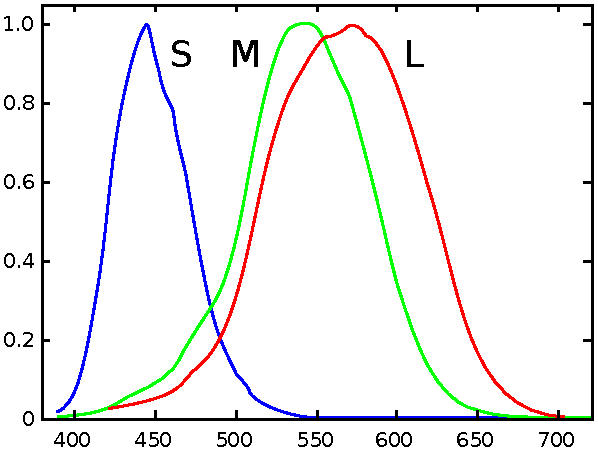
\includegraphics[width=8cm]{Cones_SMJ2_E.pdf}
	\caption{Senzitivita čípků L, M a S na vlnové délky viditelného spektra.}
	\label{fig:cones}
	\end{figure}

  Každý viditelný objekt odráží, ohýbá nebo emituje elektromagnetické vlnění z viditelné části spektra.
  Funkce hustoty vlnových délek, které viditelný objekt do oka přenáší -- ať už jako primární či sekudární zdroj -- objektivně popisuje, jakou barvou bude daný objekt vnímán.
  Napříkad funkce hustoty vlnových délek zeleného objektu bude mít většinu enegrie koncentrovanou v intervalu $\langle495; 570 \rangle$ nm.
  Lidské oko toto rozložení pronásobí se senzitivitou jednotlivých čípků a integrály odešle do mozku jako tři zmíněné hodnoty L, M a S.

  Jelikož je tato komprese ztrátová, nelze z hodnot LMS zrekonstruovat původní spektrální distribuci.
  Z toho plyne, že různé spektrální distribuce se můžou namapovat na stejnou trojici LMS, zobrazení tedy není injektivní.
  Tento efekt se nazývá metamerismus a je využíván v každodenním životě.
  Znamená to, že k reprodukci barvy, kterou má nějaký objekt, není třeba původní rozložení vlnových délek, ale pouze takové rozložení, které v lidském oku vyvolá stejnou reakci čípků LMS. \cite{Abraham2016}

  Z toho však může plynout problém, kdy můžou dva objekty reflektující světlo vyvolávat identickou reakci čípků LMS při jednom osvětlení, ale zároveň se můžou jevit naprosto odlišně při jiném osvětlení.
  Objekty, které světlo pouze emitují (dokonale černá tělesa), tímto jevem nedisponují, avšak taková tělesa se v přírodě nevyskytují.
  Tento problém se částečně řeší standardizací osvětlovacích modelů, která je rozebrána v jedné z následujících kapitol.

  \subsection{Imaginární barvy}
  Reakce čípků na vlnové délky se částečně překrývá.
  Pro každé rozložení vlnových délek světla existuje nějaká trojice LMS,
  avšak ne pro každý tristimulus existuje rozložení vlnových délek, která by takovou trojici dokázala vygenerovat.
  Relace rozložení vlnových délek ku tristimulu tedy není surjektivní.
  Z vizualizace \ref{fig:cones} je například zřejmé, že pro žádné existující rozložení vlnových délek nelze vygenerovat trojici, kde pouze hodnota M je nenulová. \cite{VincentA}

  Barva reprezentována takovým tristimulem je označována jako imaginární a jde o barvu, která se v přírodě nemůže vyskytnout.
  Takové barvy nelze běžně vnímat okem, avšak můžou vzniknout ve vizuální mozkové kůře buď jako post-processing signálů z očí, nebo jako chybový stav při nestandardním stavu vědomí.
  Teoreticky lze nemožnou barvu reprezentovat rozložením s vlnovými délkami o záporné intenzitě.
  Z hlediska počítačové grafiky jsou nemožné barvy využívány kvůli některým praktickým vlastnostem.
  Například protože jejich skládáním lze vytvořit opět reálnou barvu.
  Objektivnímu popisu a standardizaci skládání barev se věnuje komise CIE a bude se jí věnovat zbytek tohoto textu.

  \section{Funkce spektrální světelné účinnosti -- CIE 1924}
  Funkce spektrální světelné účinnosti popisuje celkovou senzitivitu lidského oka na vlnové délky světla.
  Její vizualizace je na obrázku \ref{fig:1924}.
  Tato funkce demonstruje, že světla o různých vlnových délkách se stejnou zářivostí mají různý subjektivní jas, nebo naopak světla se stejným subjektivním jasem můžou mít jinou objektivní radianci. \cite{Abraham2016}
  Tato funkce fungovala jako základ pro funkci přiřazování barev -- CIE RGB 1931 a CIE XYZ 1931.

  \begin{figure}[h!]
	\centering
	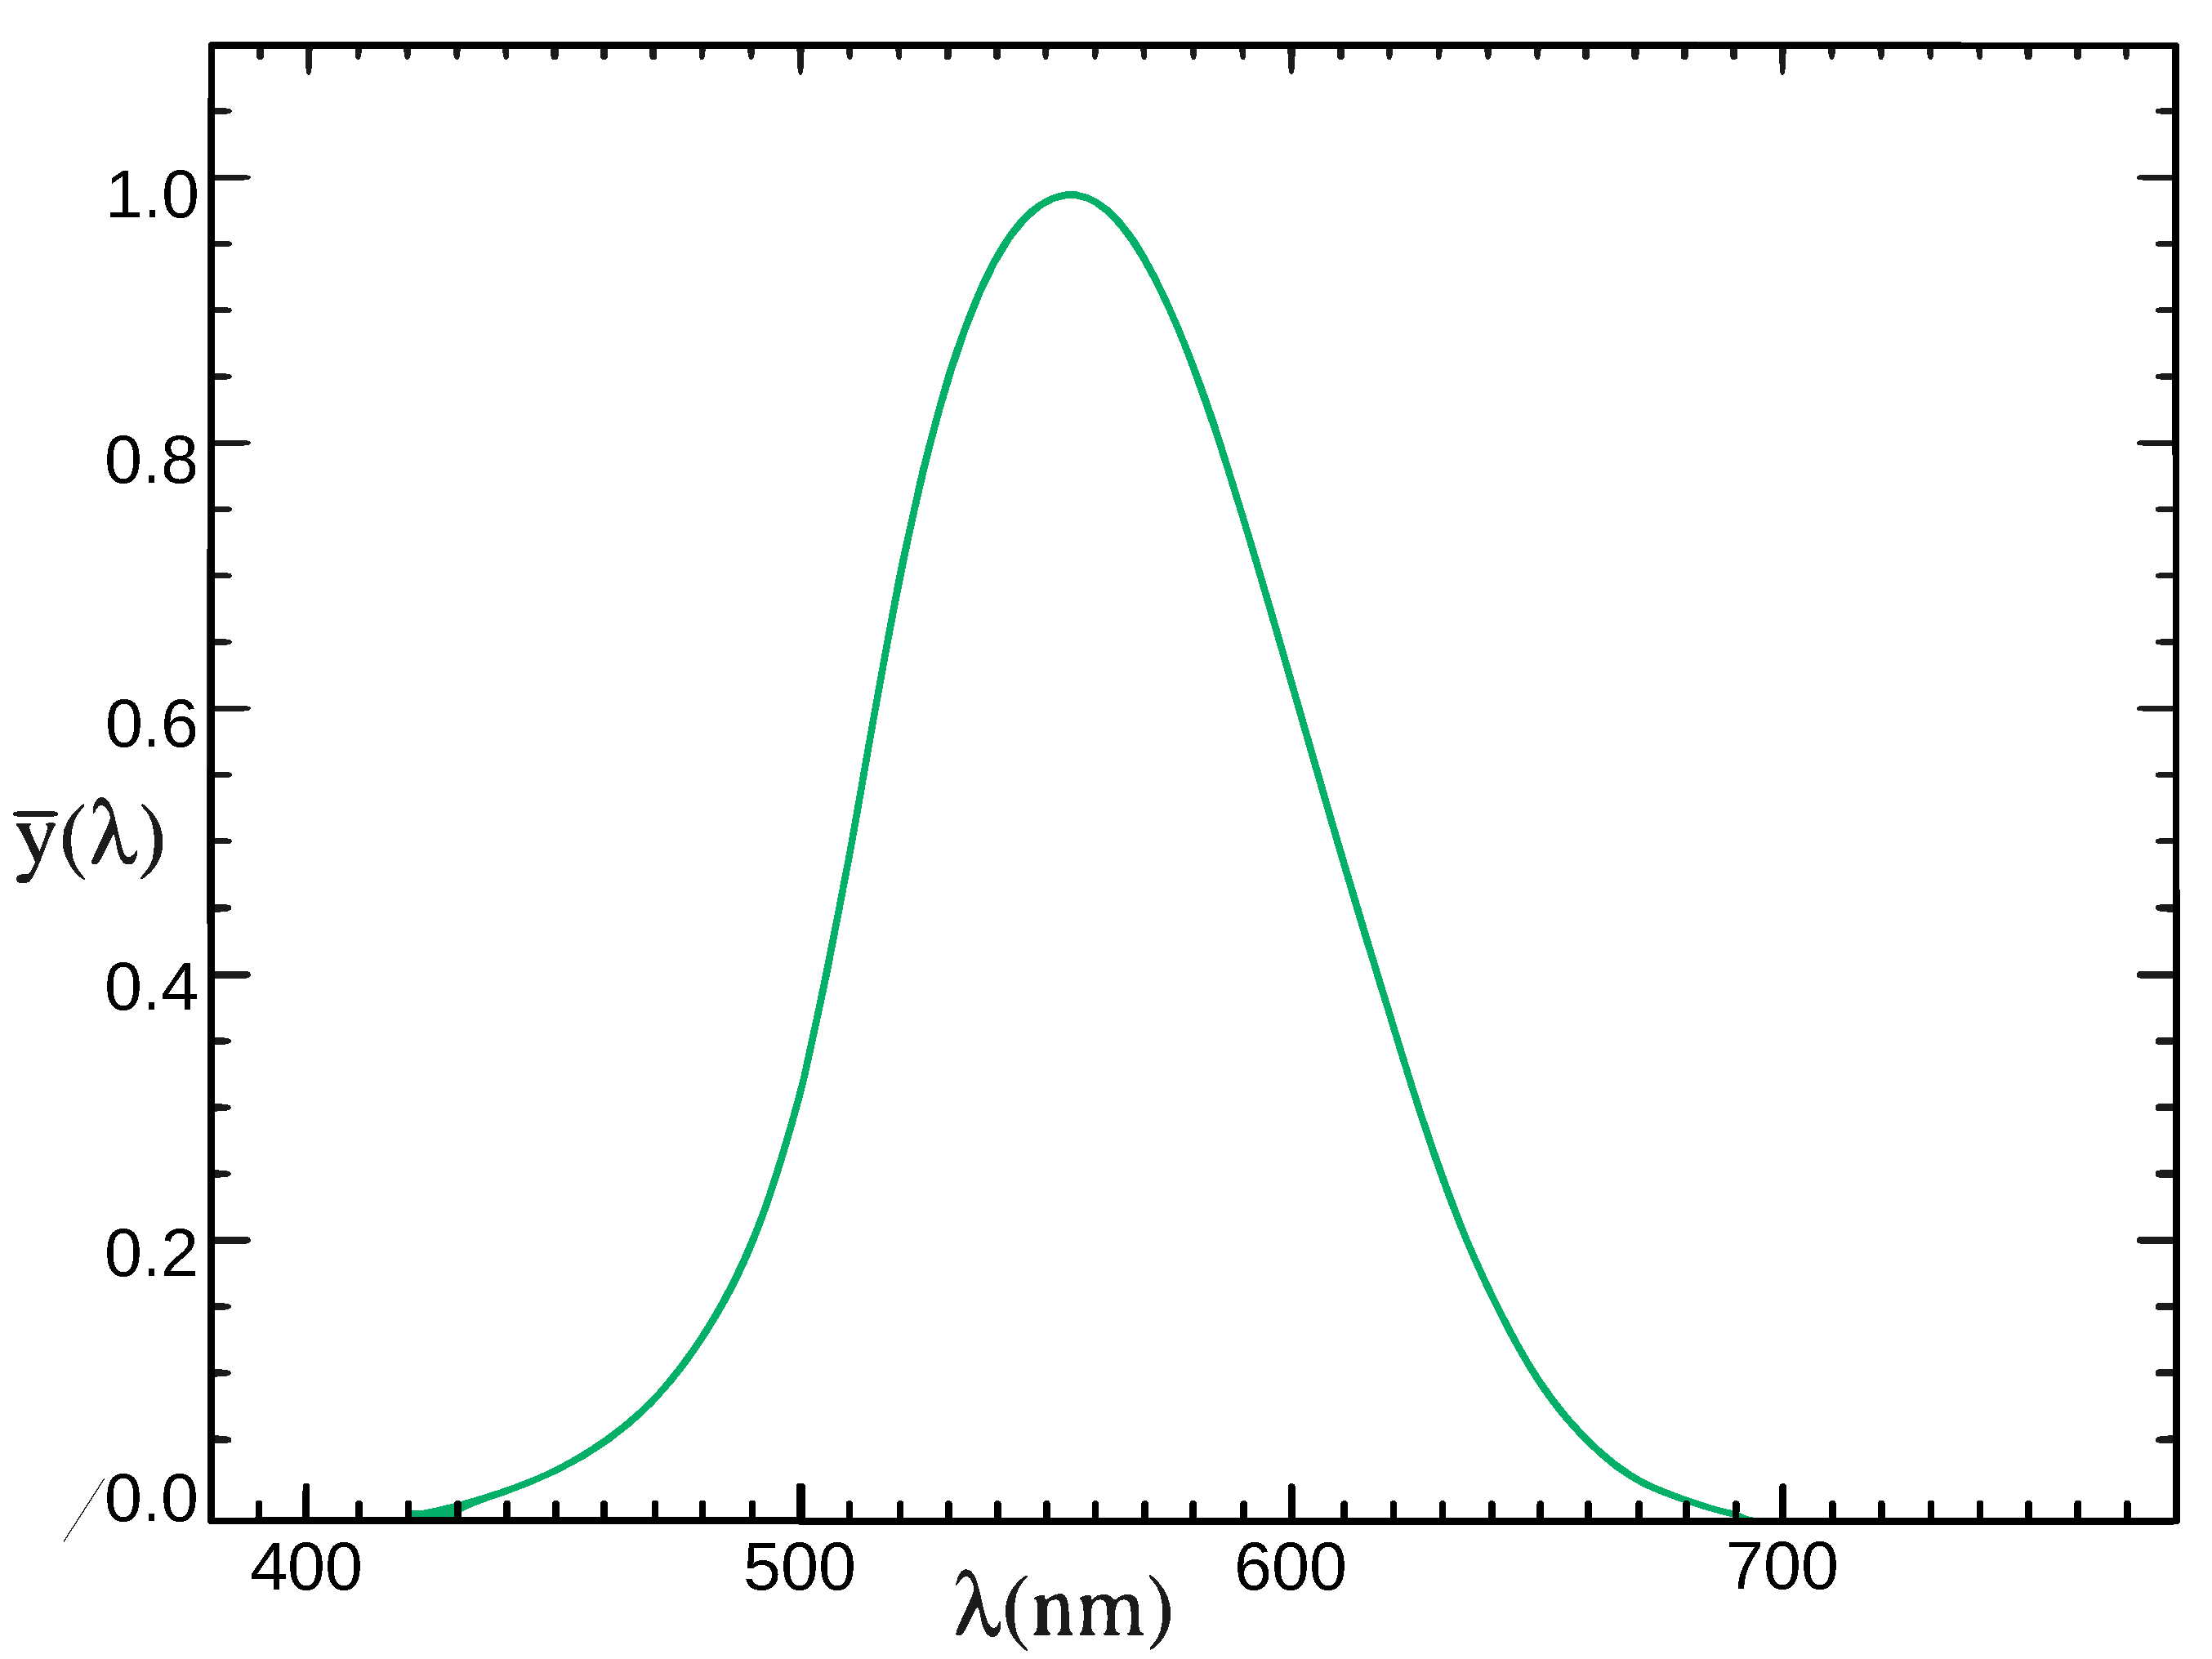
\includegraphics[width=8cm]{CIE_1931_Luminosity.pdf}
	\caption{Funkce spektrální světelné účinnosti -- CIE 1924.}
	\label{fig:1924}
	\end{figure}

  \section{Funkce přiřazování barev -- CIE RGB 1931}
  CIE RGB 1931 obsahuje trojici funkcí zvané funkce přiřazování barev RGB.
  Tyto funkce jsou postaveny nad třemi základními barvami: R (700 nm), G (546,1 nm) a B (435,8 nm).
  Vlnové délky 546,1 nm a 435,8 nm byly zvoleny jako snadno reprodukovatelné monochromatické linie rtuťové výbojky.
  Vlnovou délku 700 nm bylo v roce 1931 nesnadné reprodukovat, ale byla zvolena, protože vnímání barvy se při této vlnové délce nemění a chyby v této vlnové délce mají na výsledek malý vliv. \cite{Abraham2016, Walker1996, ciexyz}

  Tato trojice funkcí je vykreslena na obrázku \ref{fig:RGB_1931} a pro každou vlnovou délku viditelného spektra popisuje, jaký jas musí mít tři základní barvy, aby v lidském oku vznikl tristimulus odpovídající této vlnové délce.
  Funkce vykreslená na tomto obrázku je normalizovaná podle funkce spektrální světelné účinnosti -- CIE 1924, pro získání potřebné zářivosti je potřeba hodnoty ještě vynásobit odpovídající hodnotou této funkce.

  \begin{figure}[h!]
	\centering
	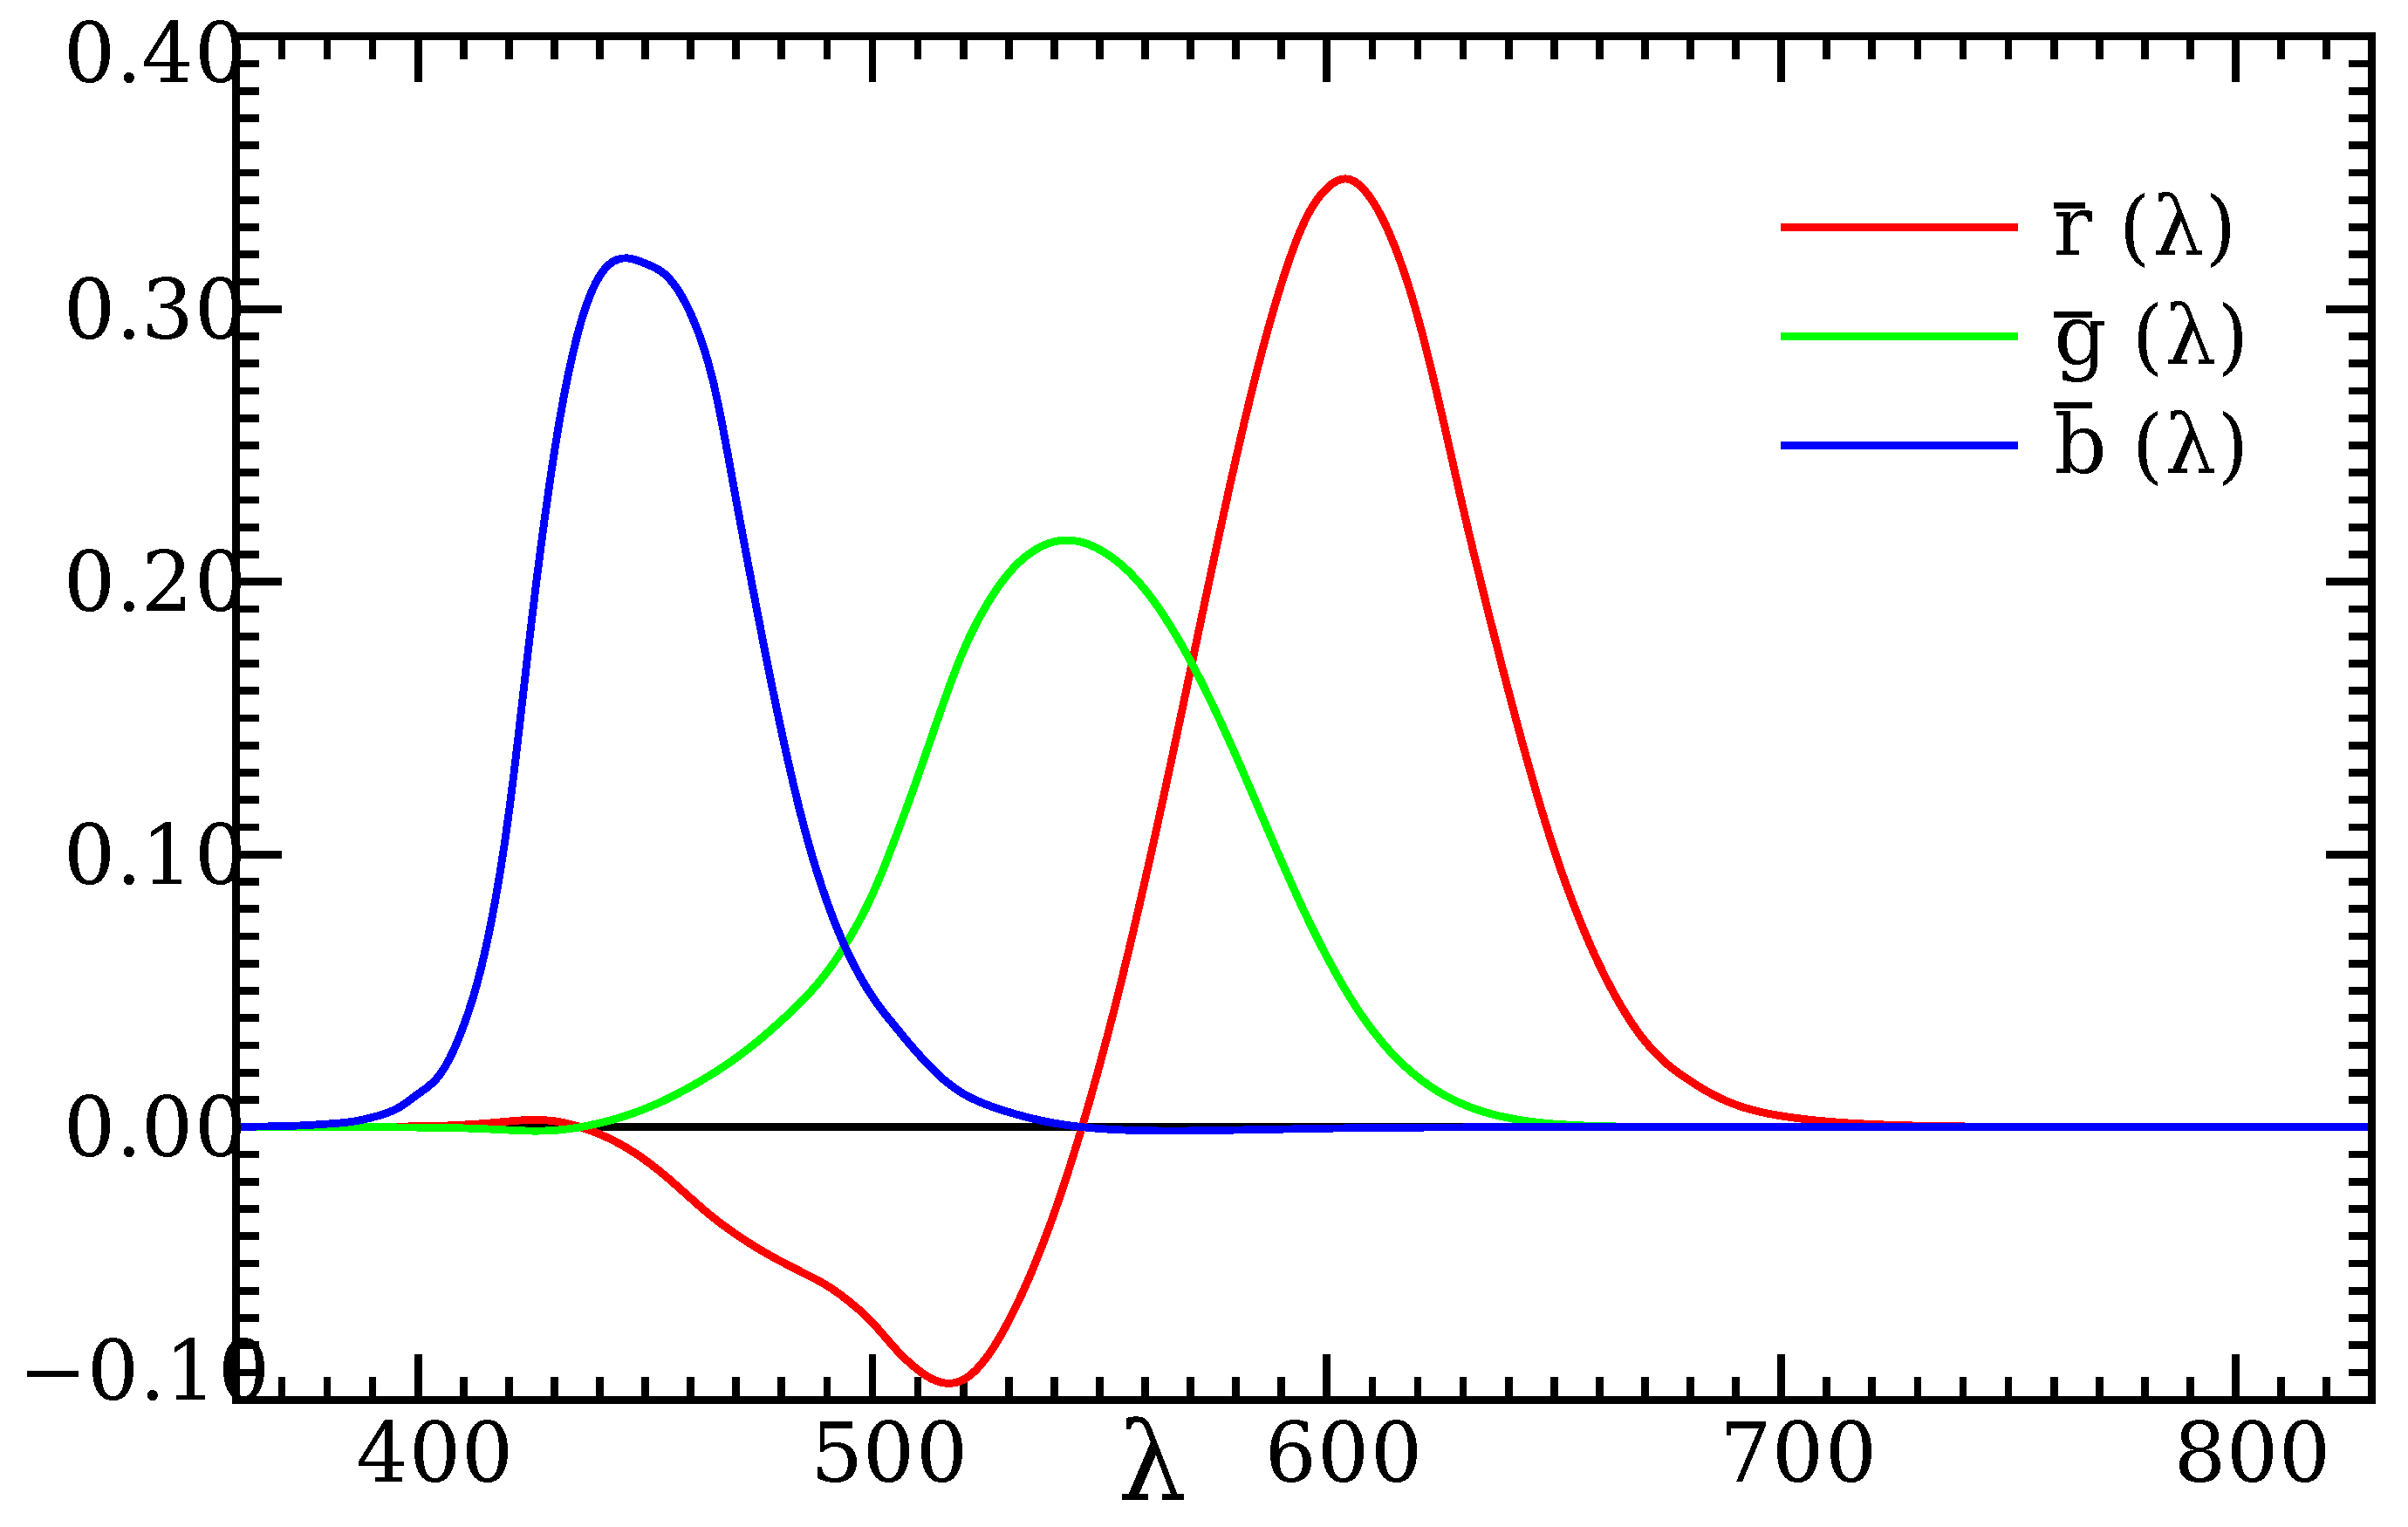
\includegraphics[width=8cm]{CIE1931_RGBCMF.pdf}
	\caption{Funkce přiřazování barev -- CIE RGB 1931.}
	\label{fig:RGB_1931}
	\end{figure}

  \subsection{Standardní pozorovatel}

  Tyto funkce byly změřeny empiricky v roce 1920 pomocí řady experimentů.
  Testovací subjekti získali na vstupu monochromatickou barvu v okénku, které zabíralo $2^\circ$ zorného pole a dostali za úkol nastavit tři potenciometry tak,
  aby lineární kombinace tří základních barev dala dohromady barvu na vstupu.
  Nastavení potenciometrů bylo zaznamenáváno jako výsledek experimentu.
  Tyto experimenty byly provedeny dvakrát nezávisle na sobě.
  Jelikož se výsledky shodovaly, byla výsledná data prohlášena za hodnoty standardního pozorovatele (CIE 1931 Standard $2^\circ$ observer). \cite{Stockman2020, ciexyz}

  Při těchto experimentech bylo zjištěno, že existují vlnové délky (520 nm), které nelze pomocí tří základních barev reprodukovat.
  S tím se v experimentech vyrovnali tak, že umožnili základní barvy přimíchávat do zdrojového monochromatického světla.
  Jakmile bylo dosaženo příslušné barvy na obou stranách, byla intenzita přimíchaných základních barev na zdroji považována za zápornou hodnotu.
  V praxi to znamená, že takovou barvu nelze v daném barevném prostoru vyjádřit, je mimo gamut. \cite{Abraham2016}

  Jelikož se později ukázalo, že experimenty s $2^\circ$ zorným polem neodpovídají vidění v běžných podmínkách, tyto experimenty byly zopakovány v roce 1964 s $10^\circ$ zorným polem (CIE 1964 Supplementary $10^\circ$ observer).

  \subsection{Chromatický diagram}

  Představit si specifickou barvu ze tří souřadnic barevného prostoru není jednoduché.
  Byl proto zaveden barevný prostor CIE rgb, který neuvažuje intenzitu barev a bere v potaz pouze chromaticitu.
  Rovnice \ref{eq:rgb} popisují převod z CIE RGB do CIE rgb.
  Výhoda těchto souřadnic je, že souřadnice leží v rovině $x + y + z = 1$.
  To znamená, že pro každé dvě hodnoty lze třetí hodnotu dopočítat.
  Diagram vykreslený ze dvou těchto souřadnic se nazývá chromatický diagram.

  \begin{align}
    \begin{split}
    r &= R / (R + G + B)\\
    g &= G / (R + G + B)\\
    b &= B / (R + G + B)
  \end{split}
    \label{eq:rgb}
  \end{align}

  Chromatický diagram pro standardního $2^\circ$ pozorovatele je vykreslen na obrázku \ref{fig:chroma_RGB_1931}.
  Každý bod na vnější křivce určuje r a g souřadnice spektrální barvy s určitou vlnovou délkou.
  Tato křivka se nazývá \textbf{lokus}.
  Každý bod uvnitř této křivky určuje souřadnice nespektrální barvy.
  Každý bod mimo tuto křivku určuje souřadnice \textbf{imaginárnách} barev.
  Základní barvy r (700 nm), resp. g (546,1 nm) spadají na souřadnice $(1, 0)$, resp. $(0, 1)$.
  Barvy ohraničené trojúhelníkem základních barev v diagramu jsou barvy, které lze vytvořit skládáním základních barev. Tato podmonožina barev se nazývá \textbf{gamut} prostoru CIE rgb.
  Barvy mimo tento trojúhelník pomocí těchto základních barev reprodukovat nelze. \cite{Abraham2016, Walker1996, ciexyz}

  Barvy v diagramu uvnitř křivky je nutno brát s odstupem.
  Nikdo neví, na jakém zařízení bude diagram zobrazen, proto jde většinou jen o hrubou aproximaci barev, které má diagram vyjařovat.
  Každé zobrazovací zařízení dokáže správně reprodukovat pouze konvexní podmonožinu barev ohraničenou souřadnicemi jeho základních barev.
  Z tvaru diagramu je zřejmé, že nemůžou existovat tři reálné základní barvy, který by pokrývaly celý prostor.

  Barvy, které jsou reprezentovány souřadnicemi uvnitř křivky jsou nespektrální barvy.
  Takové barvy lze vytvořit pouze skládáním barev spektrálních.
  Barvy na spojnici libovolných dvou bodů na křivce jsou nespektrální barvy, které lze vytvořit mícháním těchto dvou spektrálních barev.
  Z diagramu je zřejmé, že pro každou nespektrální barvu existuje nekonečně mnoho dvojic spektrálních barev, pomocí kterých lze tuto nespektrální barvu namíchat.
  V reálném světě se setkáváme zejména s nespektrálními barvami.
  Zařízení, které dokáže generovat monochromatické světlo, se nazývá laser. \cite{Abraham2016}

  \begin{figure}[h!]
	\centering
	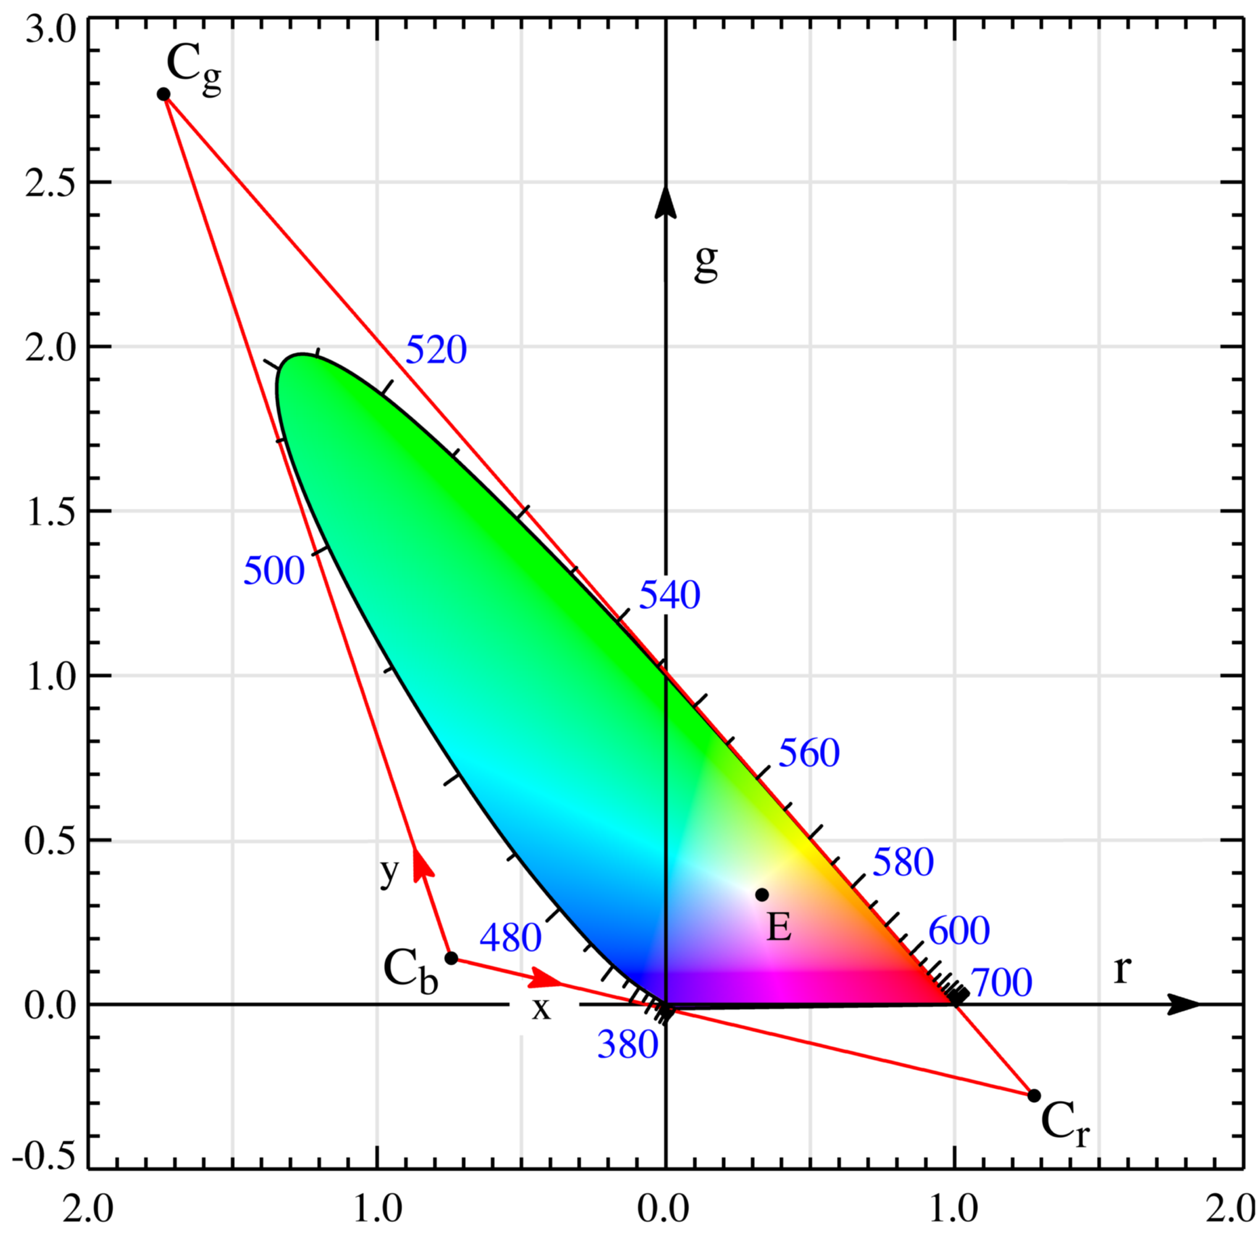
\includegraphics[width=8cm]{CIE1931_rgxy.png}
	\caption{Chromatický diagram CIE RGB 1931.}
	\label{fig:chroma_RGB_1931}
	\end{figure}

  \section{Funkce přiřazování barev -- CIE XYZ 1931}
  CIE XYZ 1931 je další trojice funkcí, která je pouze lineární transformací původního modelu CIE RGB 1931.
  Myšlenka tohoto modelu je, že jedna z funkcí může být zvolena tak, aby odpovídala funkci spektrální světelné účinnosti -- CIE 1924 V$(\lambda)$.
  To znamenená, že jas libovolné barvy může být okamžitě získán jako hodnota jedné ze složek. \cite{Abraham2016}

  Další velká výhoda tohoto modelu je, že všechny reálné barvy se nachází na kladných souřadnicích XYZ.
  Aby toho však bylo možno dosáhnout se třemi základními barvami, bylo nutno za základní barvy zvolit barvy imaginární.
  To je možné vidět na chromatickém diagramu \ref{fig:chroma_RGB_1931}, kde body C$_r$, C$_g$ a C$_b$ demonstrují základní barvy modelu CIE xyz. Chromatický diagram CIE xy po transformaci je zobrazen na obrázku \ref{fig:chroma_XYZ_1931}, kde je naopak znázorněn gamut modelu CIE rgb.
  Jelikož je CIE XYZ pouze lineární transformací, vyjadřuje naprosto stejná data a modely lze mezi sebou libovolně převádět.
  Podobně lze vykreslit i transformovanou funkci přiřazování barev. Ta je na obrázku \ref{fig:CIE_1931_XYZ_Color_Matching_Functions}. Matice pro transformaci mezi modelem CIE RGB a CIE XYZ se nacházejí v rovnici \ref{eq:rgb2xyz}. \cite{Abraham2016, Walker1996, ciexyz}

  \begin{figure}[h!]
	\centering
	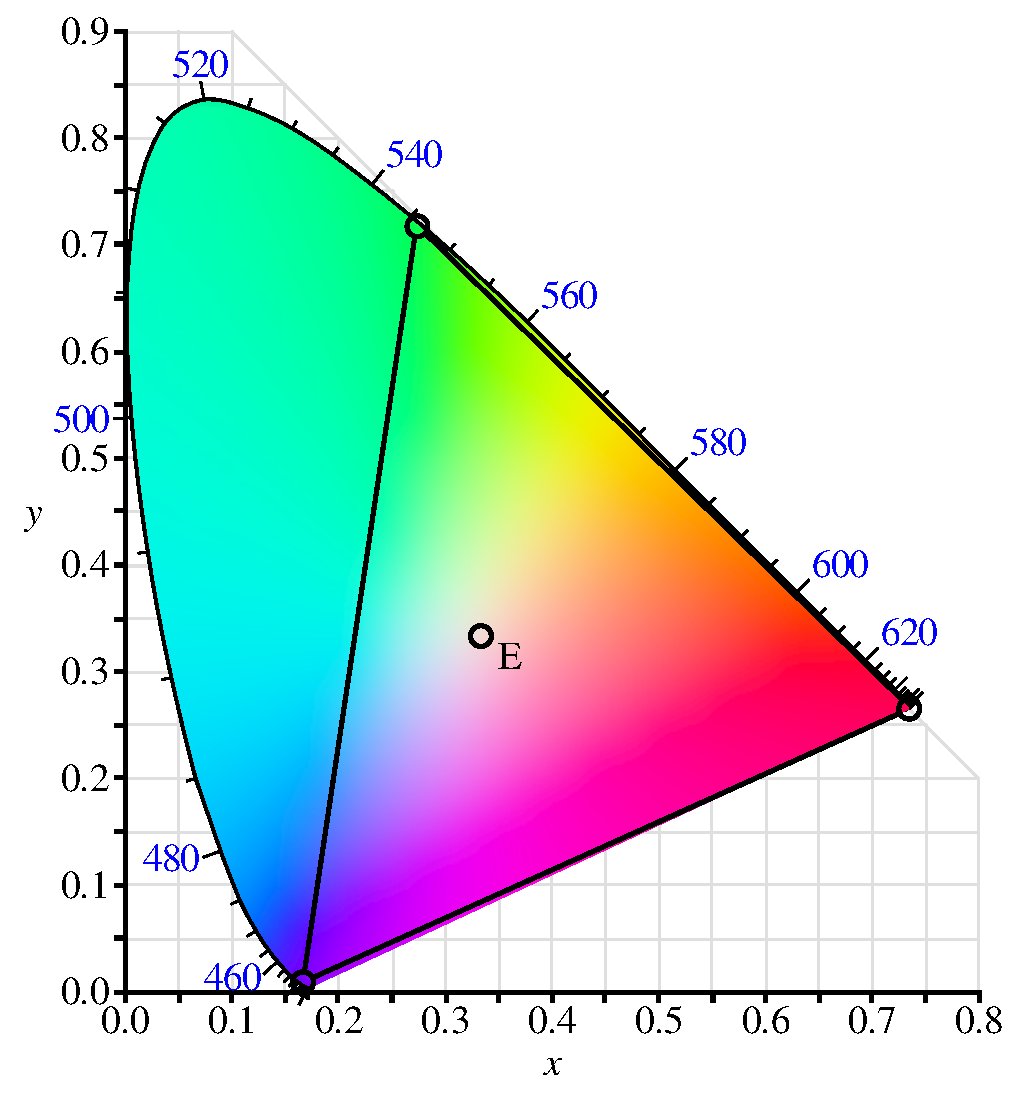
\includegraphics[width=8cm]{CIE1931xy_CIERGB.pdf}
	\caption{Chromatický diagram CIE XYZ 1931.}
	\label{fig:chroma_XYZ_1931}
	\end{figure}

  \begin{figure}[h!]
	\centering
	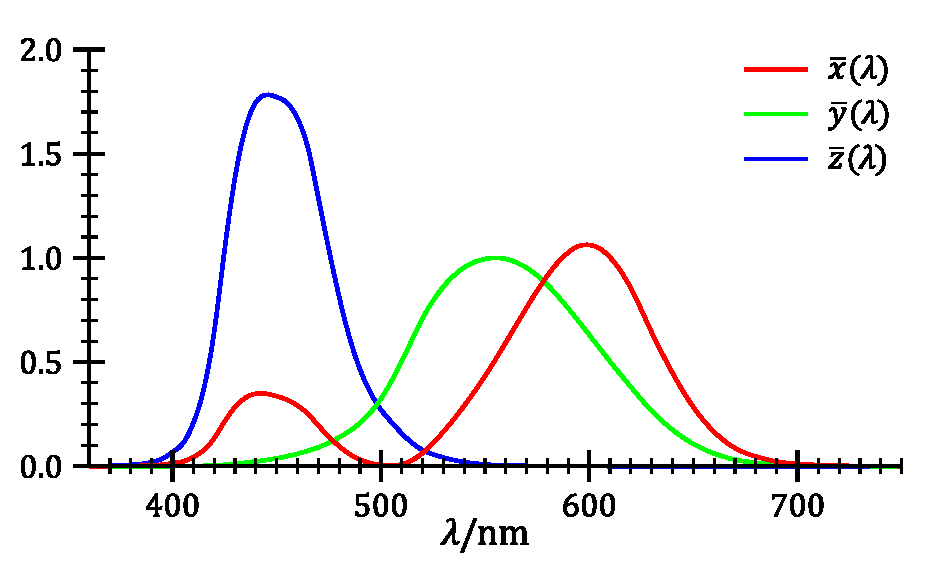
\includegraphics[width=8cm]{CIE_1931_XYZ_Color_Matching_Functions.pdf}
	\caption{Funkce přiřazování barev -- CIE XYZ 1931.}
	\label{fig:CIE_1931_XYZ_Color_Matching_Functions}
	\end{figure}

  \begin{align}
    \begin{bmatrix}
      X\\
      Y\\
      Z\\
    \end{bmatrix}
    =
    \begin{bmatrix}
      2,768 & 1,751 & 1,130\\
      1,000 & 4,590 & 0,060\\
      0,000 & 0,056 & 5,594\\
    \end{bmatrix}
    *
    \begin{bmatrix}
      R\\
      G\\
      B\\
    \end{bmatrix}
    \label{eq:rgb2xyz}
  \end{align}

  CIE XYZ slouží jako základ pro všechny ostatní barevné modely.
  Díky dobrým vlastnostem modelu CIE XYZ se model CIE RGB v praxi nepoužívá.
  S funkcemi standardního pozorovatele se pracuje v podobě transformované do CIE XYZ a všechny prakticky používané barevné podmodely jsou definované v kontextu modelu CIE XYZ.
  Z toho plyne, že pro libovolný reálně použitelný barevný model stačí definovat matice pro transformaci mezi tímto prostorem a prostorem CIE XYZ.
  Pokud požadovaná barva bude mít po transformaci kladné souřadnice, znamená to, že je vyjádřitelná v daném barevném modelu.
  Pokud bude mít navíc tento model reálné základní barvy, je možné tuto barvu v reálném světě pomocí zdrojů generujících tyto základní barvy reprodukovat. \cite{Abraham2016}

  \section{Prakticky používané barevné prostory}
  Existuje nesčetně mnoho barevných prostorů.
  Každé záznamové a zobrazovací zařízení, u kterého je požadavek na správnou reprezentaci barev, musí mít přesně definovaný barevný prostor závislý na použité technologii.
  Zároveň však existují barevné prostory, které jsou určeny pouze pro digitální zpracování.

  \subsection{sRGB}
  Každý pravděpodobně někdy pracoval s RGB daty.
  Tato data však nejsou zakódována v modelu CIE RGB 1931.
  Taková data s největší pravděpodobností referují na prostor sRGB, který vyvinul Microsoft v roce 1996.
  Matice pro převod mezi CIE XYZ a sRGB je v rovnici \ref{eq:xyz2srgb}.

  \begin{align}
    \begin{bmatrix}
      R_{\mathrm{lin}}\\
      G_{\mathrm{lin}}\\
      B_{\mathrm{lin}}\\
    \end{bmatrix}
    =
    \begin{bmatrix}
       3,2410 & -1,5374 & -0,4986\\
      -0,9692 &  1,8760 &  0,0416\\
       0,0556 & -0,2040 &  1,0570\\
    \end{bmatrix}
    *
    \begin{bmatrix}
      X\\
      Y\\
      Z\\
    \end{bmatrix}
    \label{eq:xyz2srgb}
  \end{align}

  Tato transformace však není kompletní převod.
  Aby bylo možné minimalizovat počet potřebných bitů na vzorek a zároveň správně využít citlivosti lidského oka, byla zavedena gamma korekce.
  Ta se pro prostor sRGB provádí podle rovnice \ref{eq:gamma}.
  Gamma korekce nemění informace uložené v datech.
  Jde pouze o jiné kódování těchto dat.
  Pro správné zobrazení obrázku s gamma korekcí je proto nutné provést inverzní korekci.
  Pro korektní práci s sRGB daty je také nutné nejdříve provést inverzní korekci.
  Když se například sečtou dvě barvy o stejné intenzitě, očekává se, že výsledná barva bude mít dvojnásobnou intenzitu.
  Toho lze jen těžko dosáhnout v nelineárním prostoru s gamma korekcí. \cite{srgb}

  \begin{equation}
    C = \left\{
    \begin{array}{ll}
       12.92C_{\mathrm{lin}} & C_{\mathrm{lin}} \leq 0,0031308\\
       (1 + 0,055)C_{\mathrm{lin}}^{1/2,4} - 0,055 & C_{\mathrm{lin}} > 0,0031308\\
    \end{array}
    \right.
    \label{eq:gamma}
  \end{equation}

  Model sRGB ve chromatickém diagramu CIE xy je na obrázku \ref{fig:CIExy1931_sRGB}.
  Vrcholy trojúhelníku znázorňují tři základní barvy modelu sRGB.
  Prostor uvnitř trojúhelníku jsou barvy reprodukovatelné modelem sRGB.
  Tento prostor se nazývá gamut prostoru sRGB.
  Bod D65 definuje souřadnice bílé barvy v tomto modelu. \cite{Walker1996, srgb}

  \begin{figure}[h!]
  \centering
  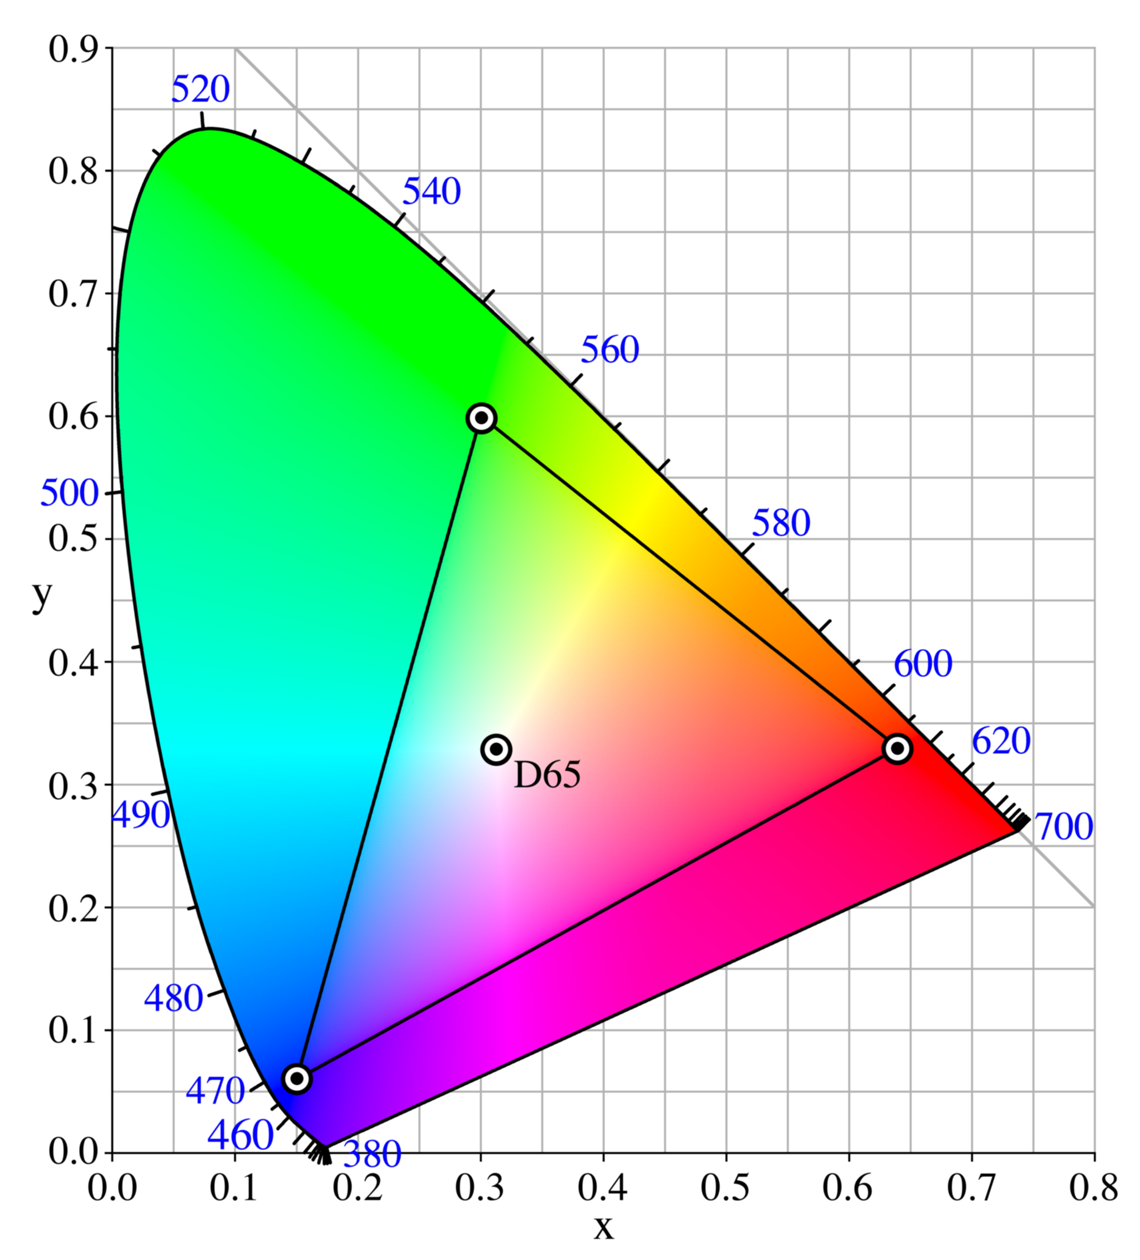
\includegraphics[width=8cm]{CIExy1931_sRGB.png}
  \caption{Gamut prostoru sRGB.}
  \label{fig:CIExy1931_sRGB}
  \end{figure}

  \subsection{Adobe RGB}
  Adobe RGB vznikl v roce 1998.
  Tento barevný prostor disponuje větším rozsahem barev.
  Červená a modrá základní barva je identická s prostorem sRGB, avšak zelená složka má hodnoty posunuty tak, aby měl tento prostor větší rozsah, jak je zobrazeno na obrázku \ref{fig:CIExy1931_AdobeRGB}.
  Adobe RGB se využívá v profesionální fotografii a zpracování videa.
  Existují monitory, které tento prostor dokáží zobrazit.

  \begin{figure}[h!]
  \centering
  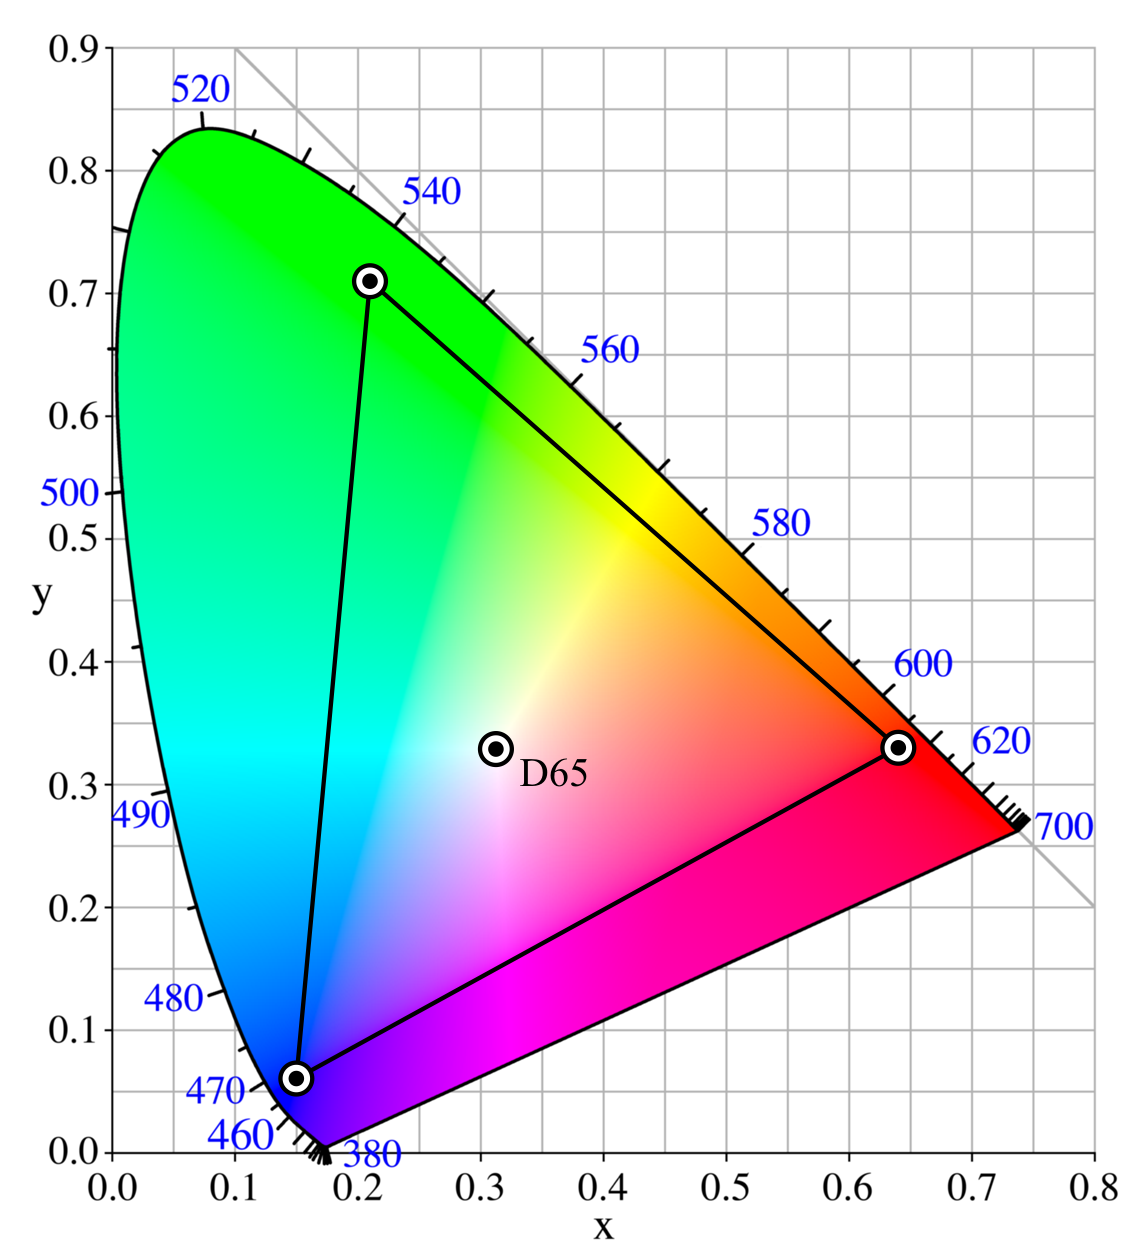
\includegraphics[width=8cm]{CIExy1931_AdobeRGB.png}
  \caption{Gamut prostoru Adobe RGB.}
  \label{fig:CIExy1931_AdobeRGB}
  \end{figure}

  \subsection{Jiné barevné prostory}
  Existuje mnoho dalších barevných prostorů.
  Za zmínku stojí například prostor Wide Gamut RGB.
  Ten pokrývá ještě větší rozsah reálných barev, než předchozí dva prostory, avšak za cenu toho, že dvě z jeho reálných barev jsou imaginární.

  Z barevných prostorů, které nevyužívají tři základní barvy, se používá například CMYK.
  Pro tento prostor však nejsou standardizovány transformace pro převod do CIE XYZ, takže namísto barevného prostoru definuje spíše způsob míchání barev.
  Využití tohoto barevného modelu je zejména v tisku.

  \section{Standardní světelný zdroj}
  Aby mohla být získána kompletní objektivní reprezentace barvy reálného tělesa, musí být kromě funkce spektrální odrazivosti/lámavosti a funkce přiřazovaných barev pozorovatele známý také osvětlovací model.
  Byla proto společností CIE standardizována řada světelných zdrojů pokrývající řadu světelných podmínek.
  Spektrální rozložení standardních světelných zdrojů A, B a C je vykreslena na obrázku \ref{fig:CIE_illuminants_A,B,C}.

  Světelný zdroj A reprezentuje klasické domácí osvětlení wolframovým vláknem o teplotě 2856~K.
  Světelné zdroje B a C jsou modifikacemi zdroje A pomocí barevných filtrů.
  Tyto zdroje mají napodobovat denní světlo.
  Zdroj B měl reprezentovat polední sluneční světlo s teplotou 4874~K, zatímco zdroj C reprezentoval denní světlo s teplotou 6774~K.
  Zdroje B a C se však ukázaly jako nepřesné a byly nahrazeny zdroji z rodiny D. \cite{stdilum}

  \begin{figure}[h!]
	\centering
	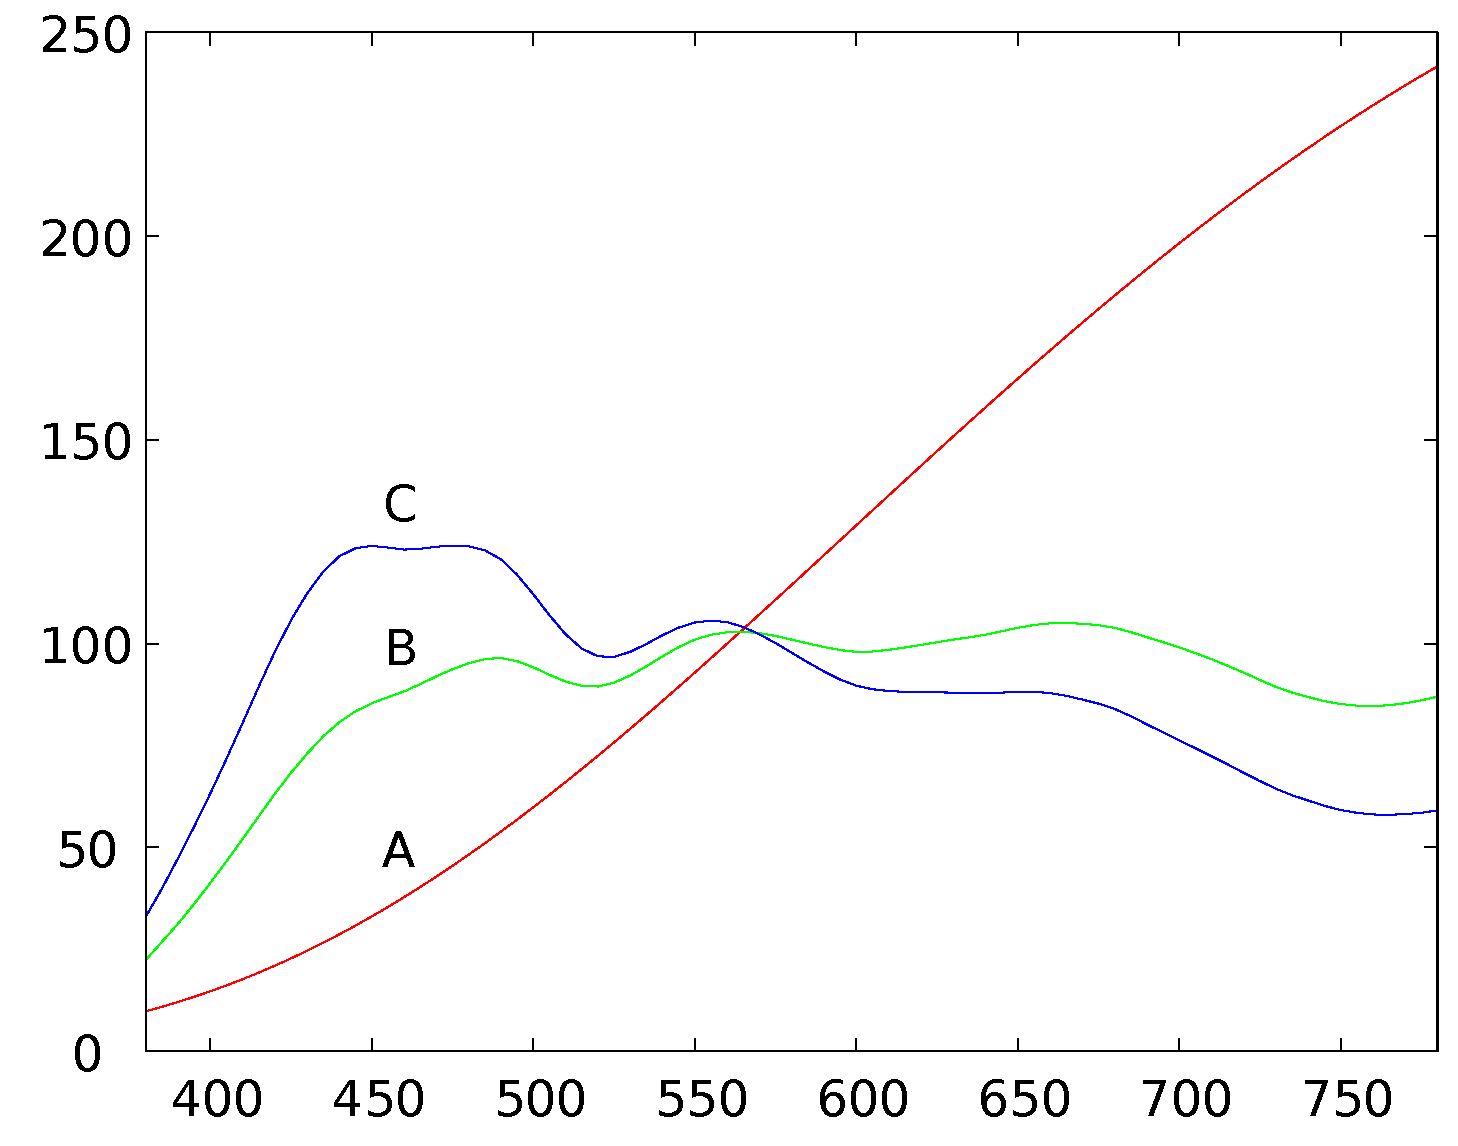
\includegraphics[width=8cm]{CIE_illuminants_A,B,C.pdf}
	\caption{Standardní světelné zdroje A, B a C.}
	\label{fig:CIE_illuminants_A,B,C}
	\end{figure}

  Zdroje z rodiny D mají reprezentovat denní světlo v různých podmínkách. Tyto zdroje není lehké vytvořit uměle.
  Myšlenka těchto zdrojů je, že spektrální distribuci denního světla lze vytvořit lineární kombinací tří fixních spektrálních distribucí, rovnice \ref{eq:d}.
  Vektor $S_0$ reprezentuje průměr všech vzorků spektrálního rozložení.
  Vektor $S_1$ reprezentuje variaci modré a žluté, která je způsobena absencí nebo přítomností mraků v přímém slunečním světle.
  Vektor $S_2$ reprezentuje variaci růžové a zelené, která je způsobena množstvím vodní páry v atmosféře.
  Tyto tři vektory jsou zobrazeny v obrázku \ref{fig:CIE_illuminants_D_components}.
  Pro rekonstrukci osvětlovacího modelu za jistých světelných podmínek je potřeba znát pouze koeficienty $M_1$ a $M_2$.
  Z rodiny D je specifikován například zdroj D50, který odpovídá teplotě ~5000~K, D55 odpovídající teplotě ~5500~K a D65 s teplotou ~6500~K.  \cite{Walker1996, stdilum}

  \begin{equation}
    S(\lambda) = S_0(\lambda) + M_1S_1(\lambda) + M_2S_2(\lambda)
    \label{eq:d}
  \end{equation}

  \begin{figure}[h!]
	\centering
	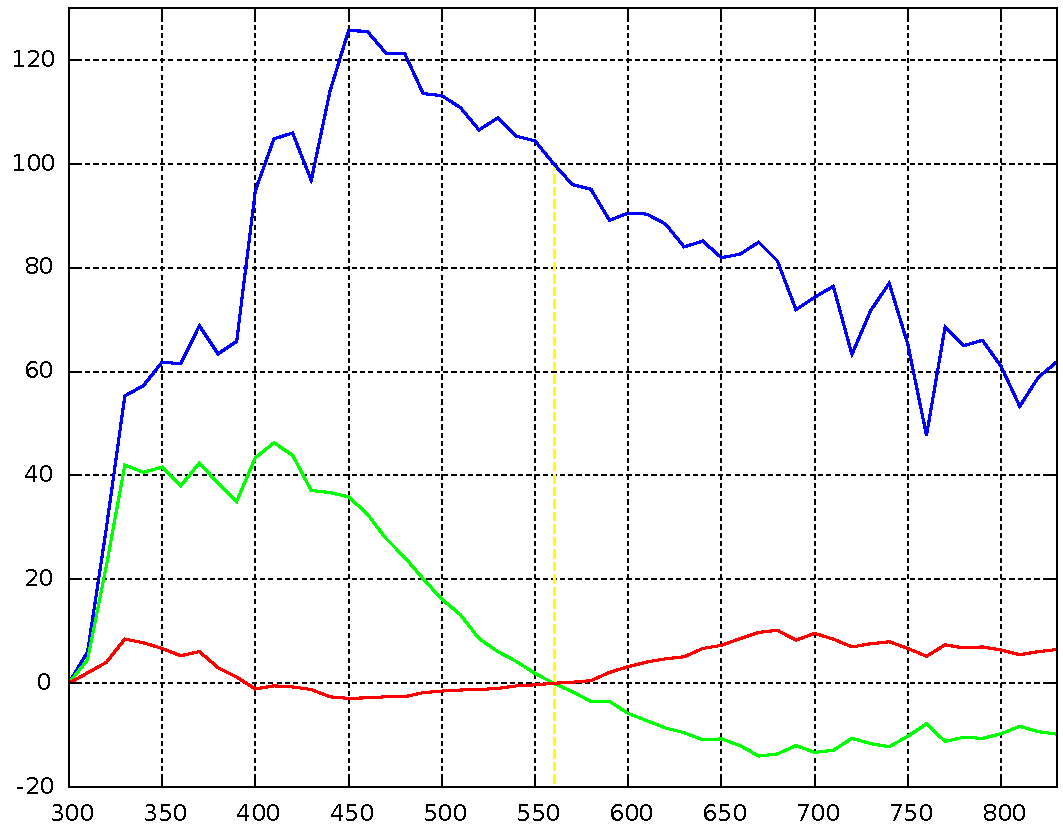
\includegraphics[width=8cm]{CIE_illuminants_D_components.pdf}
	\caption{Komponenty standardního světelného zdroje D.}
	\label{fig:CIE_illuminants_D_components}
	\end{figure}

  \section{Nástroj pro vizualizaci chromatického diagramu}
  Cílem tohoto projektu z hlediska implementačního bylo vytvořit aplikaci, která bude vizualizovat chromatický diagram.
  Aplikace, společně s tímto textem, je určena zejména pro ty, kteří mají problém problematiku míchání barev pochopit.
  Aplikace v reálném čase generuje a vykresluje chromatický diagram podle zadaných parametrů.
  Aplikace umožňuje jednoduchou kalibraci barev na použité zobrazovací zařízení tak, aby barvy spadající do kalibrovaného barevného prostoru byly věrně zobrazeny.
  Aplikace podporuje kalibraci pro barevné prostory sRGB, Adobe RGB a CIE RGB, přičemž první dva nejlépe aproximují prostory, které jsou využívané v počítačových monitorech.
  Prostor CIE RGB byl přidán pouze pro účely experimentování, není známo zobrazovací zařízení, které by tento prostor podporovalo.
  Mimo barevný prostor je možnost nastavit si také koeficient gamma korekce, který dané zobrazovací zařízení používá.

  V základním módu aplikace vykresluje chromatický diagram CIE xy se $2^\circ$ standardním pozorovatelem.
  Scéna je však trojrozměrná a tažením myši je možné ji otáčet.
  Třetí osou je v tomto případě osa z.
  Z takového diagramu je zřejmé, že všechny body barevného prostoru CIE xyz leží v rovině $x + y + z = 1$.
  Uživatel si zároveň může udělat představu o vzdálenosti mezi jednotlivými barvami, která je v diagramu CIE xy zkreslená.

  V levém panelu lze třetí osu přepnout na Y z modelu CIE XYZ, která reprezentuje jas.
  Odemkne se tím nabídka standardních osvětlovacích modelů.
  Diagram takto reprezentuje trojrozměrné těleso všech existujících barev pod zvoleným osvětlovacím modelem.
  Toto těleso se nazývá MacAdamova limita.
  Toto těleso je vykresleno pomocí algoritmu z \cite{Perales2005}, který byl modifikován tak, aby výstupní body bylo možné efektivně triangulovat.

  V každém módu aplikace je možnost volby pozorovatele, přičemž na výběr je z $2^\circ$ a $10^\circ$ standardního pozorovatele.
  Dále je umožněno měnit rozsah vykreslených vlnových délek, jehož posuvem se diagram pro tento rozsah v reálném čase přepočítá.
  Aplikace obsahuje tlačítka pro přepnutí do základních poloh kamery, jsou to: \textbf{F}ront, \textbf{R}ight, \textbf{T}op a \textbf{I}sometric.

  Při implementaci byl kladen důraz na efektivitu a modularitu.
  Výsledný tvar diagramu je počítán z veřejně dostupných tabulek standardního pozorovatele a osvětlovacího modelu.
  Vykreslená barva je determinována až na grafické kartě na základě souřadnic CIE xyY podle matic ze specifikací použitých barevných modelů.
  Uživatelské rozhraní aplikace se nachází na obrázku \ref{fig:app}.

	\begin{figure}[h!]
	\centering
	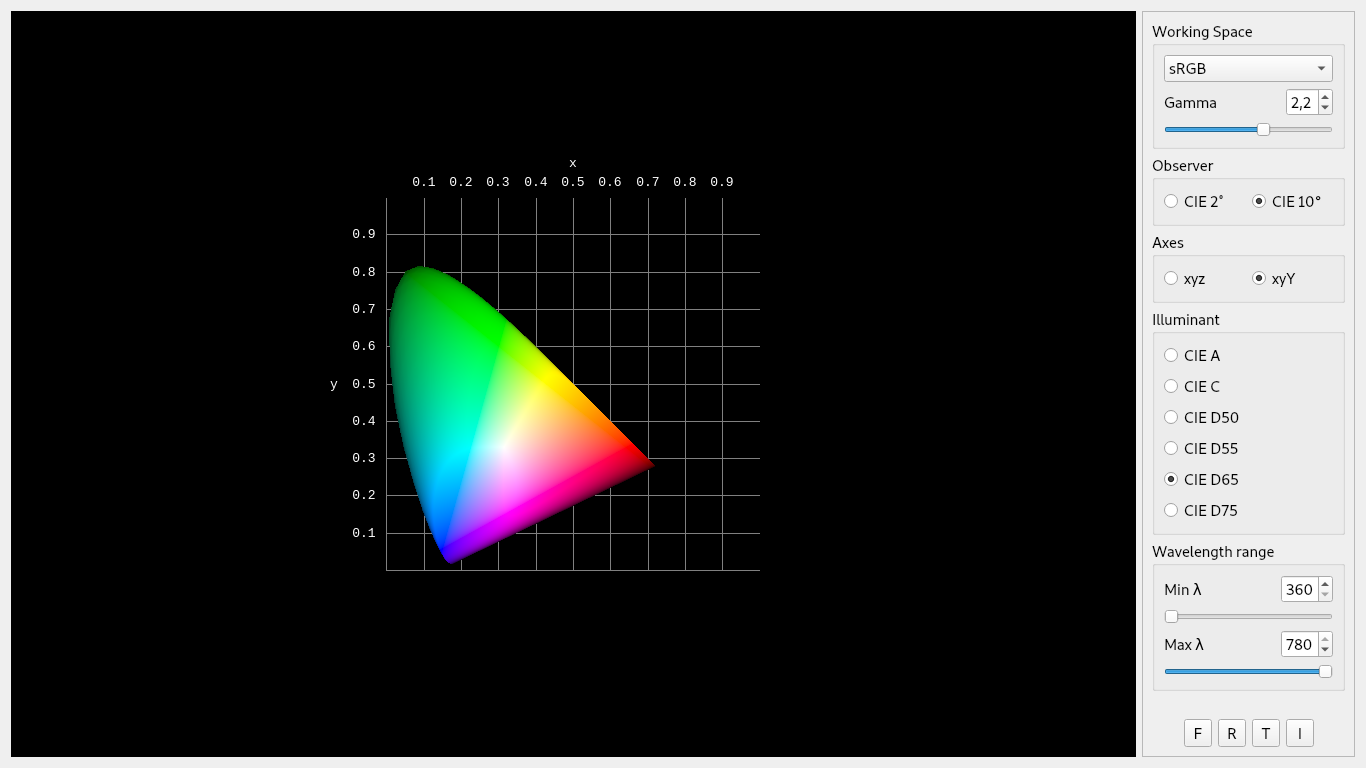
\includegraphics[width=15cm]{app.png}
	\caption{Uživatelské rozhraní aplikace.}
	\label{fig:app}
	\end{figure}

  \newpage

  \bibliographystyle{czechiso}
  \bibliography{doc}



\end{document}
